\begin{figure}[H]
    \centering
    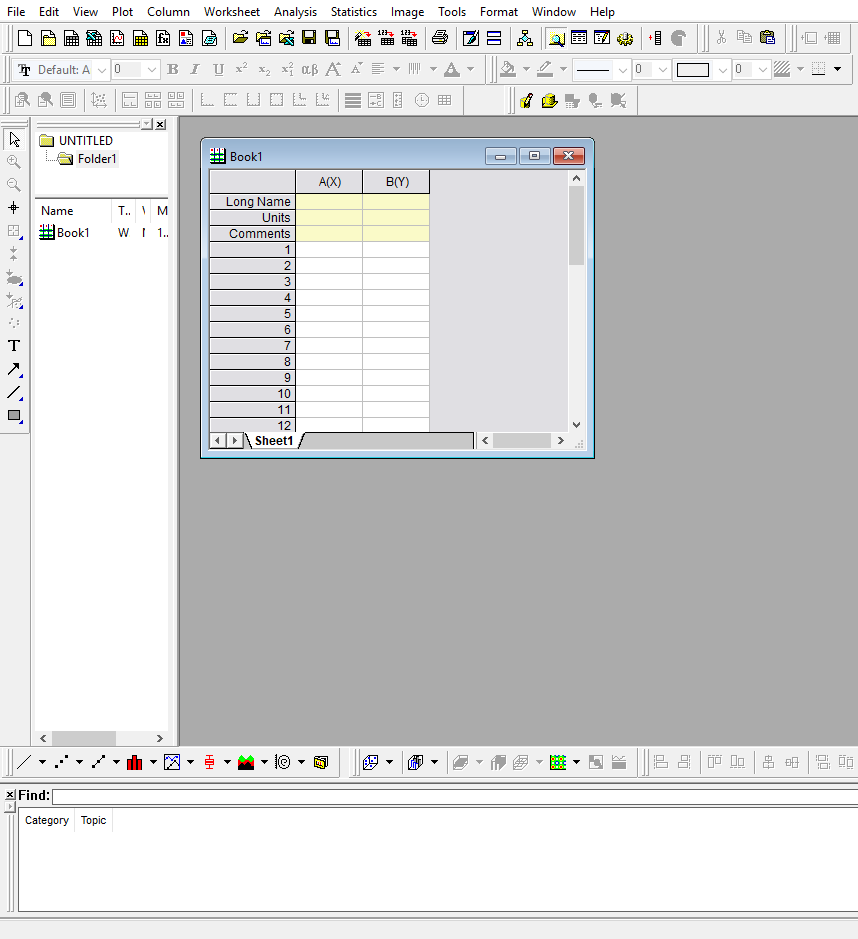
\includegraphics[width=0.8\textwidth]{basico/1mostra.png}

    \caption{Tela inicial do Origin}
    \label{fig:basico:mostragem}
\end{figure}

\subsection{Alterando a Fonte Padrão}

    Como a fonte padrão do \texttt{Origin} não funciona muito bem com acentos e outros símbolos da língua portuguesa, é recomendado utilizar outra fonte nos gráficos. Nos exemplos a seguir será aplicada a fonte \texttt{Times New Roman}, que funciona com os acentos gráficos e é facilmente encontrada em qualquer máquina com \texttt{Windows}. Todo o processo é bem simples e está especificado na figura \ref{fig:basico:mudar_fontes}.

    \begin{figure}[htbp]
        \centering
        \begin{subfigure}{0.45\textwidth}
            \centering
            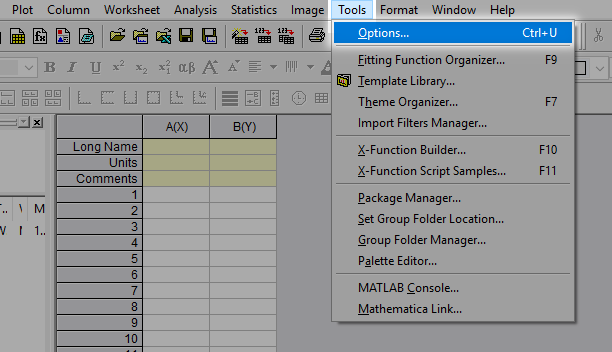
\includegraphics[width=\textwidth]{basico/2options.png}

            \caption{Acesso às opções}
            \label{fig:basico:options}
        \end{subfigure}
        ~
        \begin{subfigure}{0.45\textwidth}
            \centering
            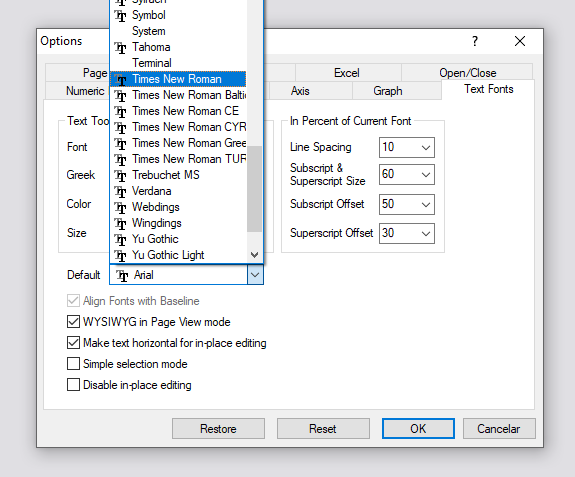
\includegraphics[width=\textwidth]{basico/3fonts.png}

            \caption{Opção de fontes}
            \label{fig:basico:fontes}
        \end{subfigure}
        \caption{Mudando a fonte padrão}
        \label{fig:basico:mudar_fontes}
    \end{figure}


\subsection{Importando os Dados}

    Os dados podem ser apenas copiados de um gerenciador de tabelas como o \texttt{Excel}, o \texttt{Google Planilhas} ou o \texttt{LibreOffice Calc} e colados na tabela do \texttt{Origin}. Quando os dados são importados assim, a formatação das linhas e colunas se matém.

    Também é possível importar dados de arquivos de texto, como os arquivos com extensão \texttt{.csv} ou planilhas salvas do \texttt{Excel}, apesar de ser um pouco mais complicado. Versões mais recentes do programa fornecem até a opção de pegar dados de páginas da \textit{internet}.

    \begin{lembrete}
        Cuidado com o separador decimal. Em português e outras línguas europeias é mais comum encontrar a vírgula [\texttt{,}] como separador da parte decimal do número, enquanto nos países anglofônicos é o ponto final [\texttt{.}] que define a parte fracionária e a vírgula serve para separar os milhares. Isso pode trazer problemas na hora de importar os dados, dependendo da configuração do \texttt{Origin} e da formatação original dos dados.
    \end{lembrete}


\subsection{Renomeando Colunas} \label{sec:basico:renome}

    Por padrão, as colunas são criadas com letras (figura \ref{fig:basico:importado}). Para mudar isso, basta alterar as propriedades da coluna (acessada com um clique duplo na coluna), como na figura \ref{fig:basico:renomear}. Os campos mais importantes são:

    \begin{description}
        \item[Short Name] o nome da coluna na tabela do \texttt{Origin}
        \item[Long Name] um nome mais descritivo para o valor e é o que normalmente aparece no gráfico
        \item[Units] a gradeza física do valor
        \item[Plot Designation] é a função da coluna no gráfico, que pode ser \texttt{Y}, \texttt{X}, \texttt{YErr}, \texttt{Z}, entre outros...
    \end{description}

    Além disso, se você importar os dados de um arquivo \texttt{CSV}, é possível utilizar as primeiras linhas como nome ou descrição da coluna.

    \begin{figure}[htbp]
        \centering
        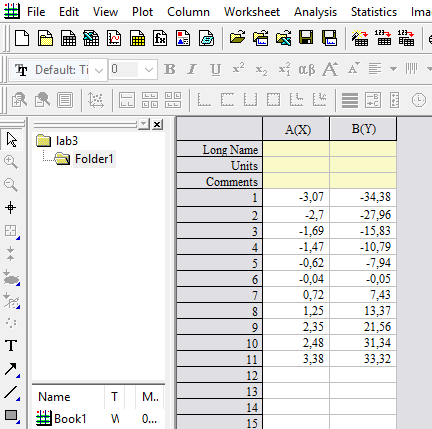
\includegraphics[width=0.7\textwidth]{basico/4import.png}

        \caption{Colunas com nomes genérico}
        \label{fig:basico:importado}
    \end{figure}

    \begin{figure}[htbp]
        \centering
        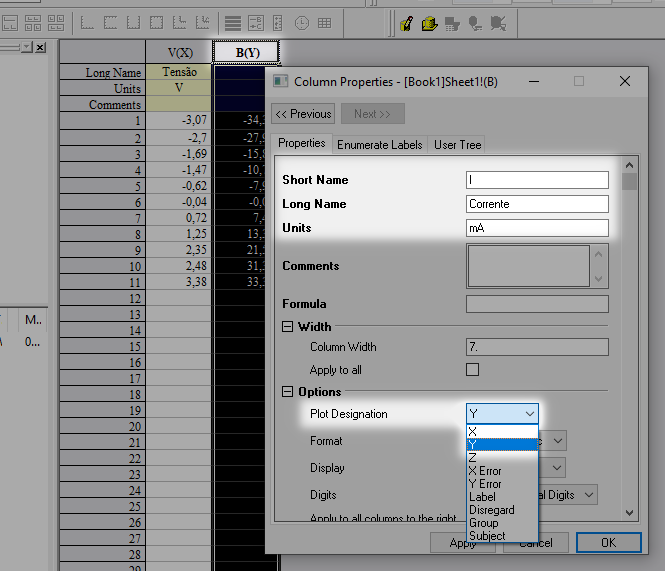
\includegraphics[width=0.8\textwidth]{basico/5renome.png}

        \caption{Alterando as propriedades da coluna}
        \label{fig:basico:renomear}
    \end{figure}
